\documentclass[11pt,a4paper]{article}
\usepackage[utf8]{inputenc}
\usepackage{amsmath,amssymb}
\usepackage{graphicx}
\usepackage{booktabs}
\usepackage{listings}
\usepackage{color}
\usepackage{tikz}
\usetikzlibrary{shapes,arrows,positioning}
\usepackage{hyperref}
\usepackage{geometry}
\usepackage{makeidx}

\makeindex

\geometry{margin=1in}
\hypersetup{
    colorlinks=true,
    linkcolor=blue,
    filecolor=magenta,      
    urlcolor=cyan,
    pdftitle={Fluidrop Technical Documentation},
    pdfpagemode=FullScreen,
}

% Code listing styles
\definecolor{mGreen}{rgb}{0,0.6,0}
\definecolor{mGray}{rgb}{0.5,0.5,0.5}
\definecolor{mPur}{rgb}{0.58,0,0.82}
\definecolor{background}{rgb}{0.97,0.97,0.98}

\lstdefinestyle{CStyle}{
    backgroundcolor=\color{background},   
    commentstyle=\color{mGreen},
    keywordstyle=\color{blue},
    numberstyle=\tiny\color{mGray},
    stringstyle=\color{mPur},
    basicstyle=\ttfamily\footnotesize,
    breakatwhitespace=false,         
    breaklines=true,                 
    captionpos=b,                    
    keepspaces=true,                 
    numbers=left,                    
    numbersep=5pt,                  
    showspaces=false,                
    showstringspaces=false,
    showtabs=false,                  
    tabsize=2,
    frame=single
}

\begin{document}

% --- COVER PAGE ---
\begin{titlepage}
    \centering
    \vspace*{0.5cm}
    
    % Logos
    \begin{figure}[h]
        \centering
        \begin{minipage}{0.45\textwidth}
            \centering
            \includegraphics[height=2.2cm]{iisclogo.png}
        \end{minipage}
        \hfill
        \begin{minipage}{0.45\textwidth}
            \centering
            \includegraphics[height=2.2cm]{omilogo.png}
        \end{minipage}
    \end{figure}
    
    \vspace{2.5cm}
    
    {\Huge\bfseries Fluidrop Electronic Pipette\par}
    \vspace{0.8cm}
    {\Large\bfseries High-Precision Volumetric Liquid Handling System\par}
    \vspace{2.5cm}
    
    {\Large\bfseries Knowledge Transfer Document\par}
    \vspace{0.5cm}
    {\large OMI Lab, IISc Bangalore\par}
    
    \vfill
    
    \begin{minipage}{0.8\textwidth}
        \centering
        \textbf{Author:} Kahaan Padiya \\
        \textbf{Under the Guidance of:} Prof. Sai Siva Gorthi \\
        \vspace{0.8cm}
        \textit{Optofluidics, Microfluidics, and Bio-Imaging (OMI) Laboratory \\
        Indian Institute of Science (IISc), Bangalore}
    \end{minipage}
    
    \vfill
    {\large \today \par}
\end{titlepage}

\newpage
\tableofcontents
\newpage

\section{System Architecture Overview}
The Fluidrop electronic pipette operates as a hybrid local/remote cyber-physical device. Local user input is processed on-board using a rotary encoder\index{rotary encoder} and software-driven SPI OLED display\index{OLED display}, while remote host communication is handled via the browser-based Web Serial API\index{Web Serial}.

\begin{figure}[htbp]
\centering
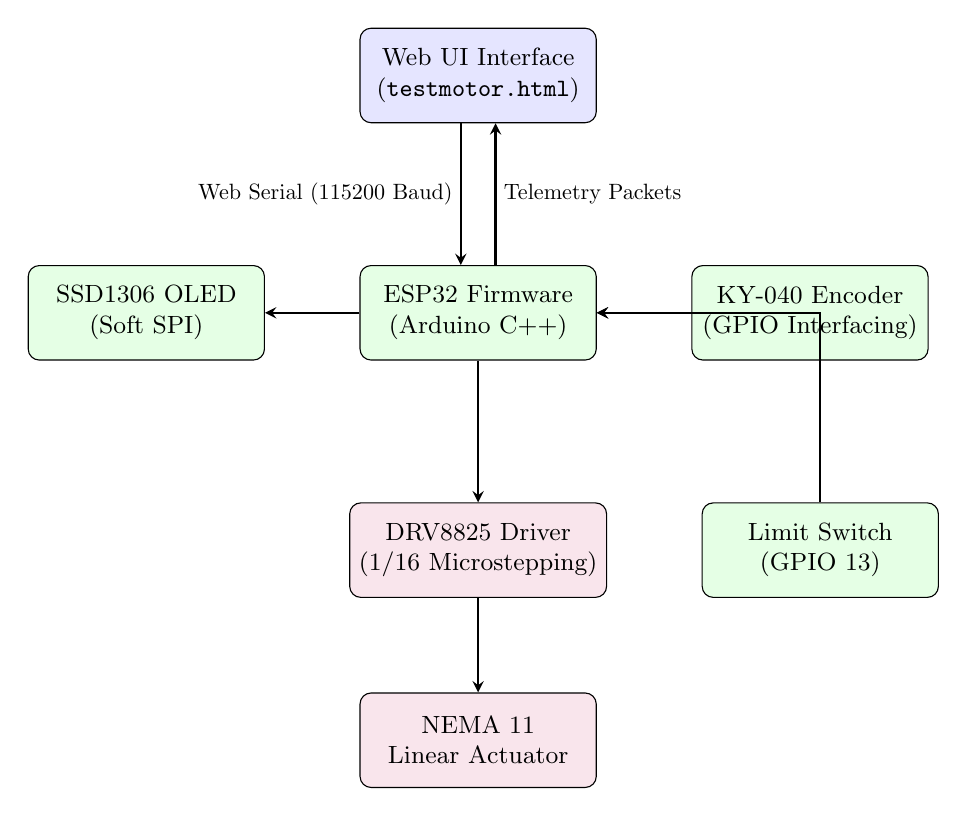
\begin{tikzpicture}[
    box/.style={draw, rectangle, rounded corners, minimum width=3cm, minimum height=1.2cm, align=center, fill=blue!10, font=\small},
    device/.style={draw, rectangle, rounded corners, minimum width=3cm, minimum height=1.2cm, align=center, fill=green!10, font=\small},
    driver/.style={draw, rectangle, rounded corners, minimum width=3cm, minimum height=1.2cm, align=center, fill=purple!10, font=\small},
    arrow/.style={->, >=stealth, thick}
]
    % Nodes
    \node[box] (web) {Web UI Interface \\ (\texttt{testmotor.html})};
    \node[device, below=1.8cm of web] (esp) {ESP32 Firmware \\ (Arduino C++)};
    \node[device, left=1.2cm of esp] (oled) {SSD1306 OLED \\ (Soft SPI)};
    \node[device, right=1.2cm of esp] (encoder) {KY-040 Encoder \\ (GPIO Interfacing)};
    \node[driver, below=1.8cm of esp] (drv) {DRV8825 Driver \\ (1/16 Microstepping)};
    \node[driver, below=1.2cm of drv] (motor) {NEMA 11 \\ Linear Actuator};
    \node[device, right=1.2cm of drv] (switch) {Limit Switch \\ (GPIO 13)};

    % Connections
    \draw[arrow] (web.250) -- node[left, scale=0.8] {Web Serial (115200 Baud)} (esp.110);
    \draw[arrow] (esp.70) -- node[right, scale=0.8] {Telemetry Packets} (web.290);
    \draw[arrow] (esp) -- (oled);
    \draw[arrow] (encoder) -- (esp);
    \draw[arrow] (esp) -- (drv);
    \draw[arrow] (drv) -- (motor);
    \draw[arrow] (switch) |- (esp);
\end{tikzpicture}
\caption{Fluidrop Hardware and Software Control Topology}
\label{fig:architecture}
\end{figure}

\section{Hardware and Mechanical Subsystems}

\subsection{Linear Actuator and Stepper Motor}
The core mechanical displacement is driven by a non-captive NEMA 11 stepper motor integrated with a high-precision lead screw\index{linear actuator}. Plunger translation relies on microstepping commands sent via the \texttt{AccelStepper} library.
\begin{itemize}
    \item \textbf{Microstepping:} The DRV8825 microstep indexer\index{DRV8825} is configured via GPIO pins \texttt{M0} (pin 25), \texttt{M1} (pin 33), and \texttt{M2} (pin 32) to \textbf{1/16 microstepping}\index{microstepping} (equivalent to 3,200 microsteps per revolution). This high resolution enables sub-microliter volumetric precision.
    \item \textbf{Plunger Travel:} The actuator slides between an open top position (zero reference) and a maximum physical stroke limit (blowout position).
\end{itemize}

\subsection{Reference Coordinate System}
The physical system utilizes three principal reference targets (measured in microsteps):
\begin{enumerate}
    \item \textbf{Home Position ($0$):} Fully retracted plunger state, serving as the system's global absolute zero reference.
    \item \textbf{First Stop ($firstStopPosition$):} The aspiration threshold coordinate. Plunger is driven here to purge air gaps prior to sample intake.
    \item \textbf{Blowout Position ($blowoutPosition$):} The lowest physical travel limit, ensuring complete purge of residual fluid.
\end{enumerate}

\subsection{Limit Switch Interfacing and Drift Compensation}
An active-low mechanical limit switch\index{limit switch} is situated at the bottom limit of the plunger mechanism, wired to GPIO 13 with internal pull-up enabled.
\begin{itemize}
    \item \textbf{Auto-Homing:} During startup, the actuator drives downward until the limit switch triggers, establishing a repeatable origin.
    \item \textbf{Real-Time Drift Calibration:} During active dispenses (\texttt{DISP} commands), the switch transition is polled. If mechanical backlash or step-slippage occurs, the position of the hit is registered:
    \begin{equation}
        \Delta_{drift} = \text{switchHitPosition} - (blowoutPosition - blowoutOffset)
    \end{equation}
    The firmware dynamically applies this offset via \texttt{setCurrentPosition()} to maintain absolute step synchronisation\index{drift compensation}.
\end{itemize}

\newpage
\section{Firmware Architecture}

\subsection{EEPROM Memory Mapping}
The ESP32 allocates 512 bytes of virtualized flash EEPROM\index{EEPROM} memory. Key parameters are mapped to static offset addresses:

\begin{table}[h]
\centering
\begin{tabular}{llcl}
\toprule
\textbf{Parameter} & \textbf{EEPROM Address} & \textbf{Size (Bytes)} & \textbf{Data Type} \\
\midrule
\texttt{firstStopPosition} & \texttt{ADDR\_FIRST\_STOP} (0) & 4 & \texttt{long} \\
\texttt{blowoutPosition} & \texttt{ADDR\_BLOWOUT} (4) & 4 & \texttt{long} \\
\texttt{stepsPerUL} & \texttt{ADDR\_STEPS\_PER\_UL} (8) & 4 & \texttt{float} \\
\texttt{maxCapacity} & \texttt{ADDR\_MAX\_CAPACITY} (12) & 4 & \texttt{float} \\
\texttt{deceleration} & \texttt{ADDR\_DECEL} (20) & 4 & \texttt{float} \\
\texttt{maxSpeed} & \texttt{ADDR\_SPEED} (186) & 4 & \texttt{float} \\
\texttt{calPoints} Array & \texttt{ADDR\_CAL\_POINTS} (26) & 160 & \texttt{CalPoint[20]} \\
\bottomrule
\end{tabular}
\caption{Firmware Memory Parameter Offsets}
\label{tab:eeprom_map}
\end{table}

\subsection{Piece-Wise Multi-Point Accuracy Calibration}
To compensate for structural barrel non-linearities, the firmware interpolates measurements using a target-versus-measured lookup array\index{calibration}. The corrected volume $V_{compensated}$ is computed using:
\begin{equation}
    V_{compensated} = V_{target} \cdot \left[ C_i + t \cdot (C_{i+1} - C_i) \right]
\end{equation}
Where $C_i = \frac{T_i}{M_i}$ represent correction coefficients for neighboring calibration points, and the interpolation weight $t$ is:
\begin{equation}
    t = \frac{V_{target} - T_i}{T_{i+1} - T_i}
\end{equation}
This piece-wise linear interpolation\index{piece-wise linear interpolation} is calculated dynamically in the firmware to modify steps target calculation on the fly.

\subsection{Serial Control Protocol API}
The firmware reads command packets terminated with a newline character. Primary commands include:
\begin{itemize}
    \item \texttt{PREP}: Move plunger to \texttt{firstStopPosition}.
    \item \texttt{VOL:<vol>}: Linearly interpolate volume to absolute coordinate target and jog motor.
    \item \texttt{DISP}: Dispense to blowout with active drift limit monitoring.
    \item \texttt{AUTO\_HOME}: Drive homing routine using the limit switch.
\end{itemize}

\section{Frontend Interface Design}
The frontend interface (\texttt{testmotor.html}) communicates with the pipette via the Google Chrome Web Serial API at 115200 baud.
\begin{itemize}
    \item \textbf{Telemetry Parser:} Reads incoming telemetry lines matching the pattern \texttt{STATE:pos,stop1,stop2,factor,capacity,speed,decel}.
    \item \textbf{Keyboard Bindings:} Listens globally for Spacebar presses (excluding focused text inputs) to trigger the main workflow loop.
    \item \textbf{Active Multipliers:} Dynamically updates the active steps/\textmu L volume factor displayed on the page header when capacity modifications or calibration changes are uploaded.
\end{itemize}

\section{Interactive System Workflows}

\subsection{Aspiration and Dispense Sequence}
The sequence diagram below displays the execution path during a standard pipetting cycle triggered via the host Web UI interface:

\begin{figure}[htbp]
\centering
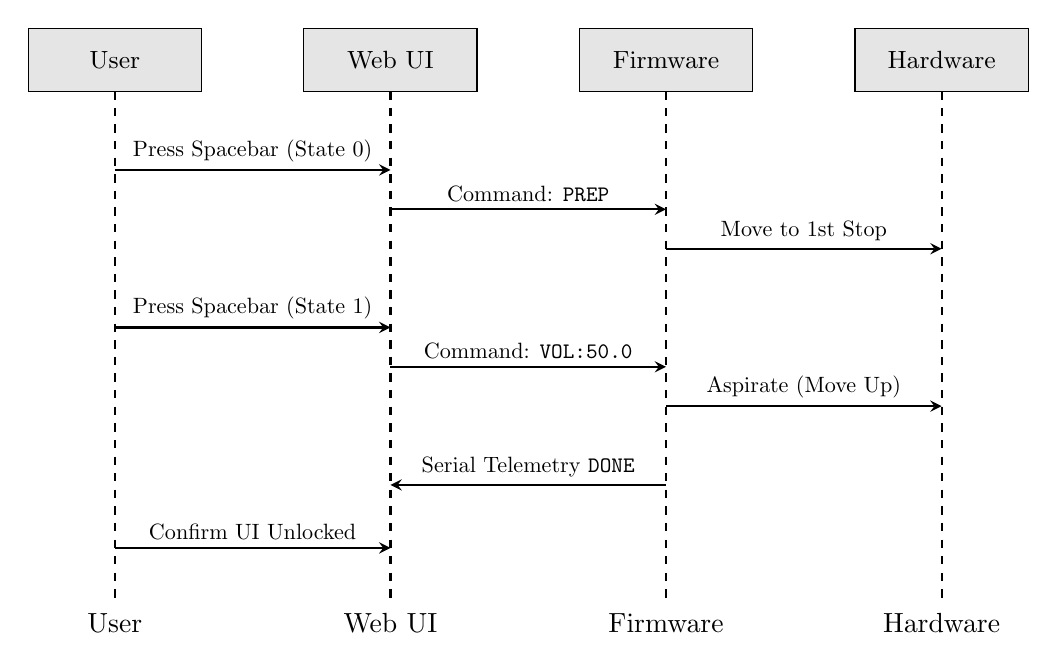
\begin{tikzpicture}[
    node distance=1.5cm and 2cm,
    line/.style={draw, thick, -latex'},
    actor/.style={draw, rectangle, minimum width=2.2cm, minimum height=0.8cm, fill=gray!20, font=\small}
]
    % Vertical lines
    \draw[dashed, thick] (0,0) -- (0,-6.5) node[below] {User};
    \draw[dashed, thick] (3.5,0) -- (3.5,-6.5) node[below] {Web UI};
    \draw[dashed, thick] (7,0) -- (7,-6.5) node[below] {Firmware};
    \draw[dashed, thick] (10.5,0) -- (10.5,-6.5) node[below] {Hardware};

    % Actor headers
    \node[actor] at (0,0.4) {User};
    \node[actor] at (3.5,0.4) {Web UI};
    \node[actor] at (7,0.4) {Firmware};
    \node[actor] at (10.5,0.4) {Hardware};

    % Message lines
    \draw[->, >=stealth, thick] (0,-1) -- node[above, scale=0.8] {Press Spacebar (State 0)} (3.5,-1);
    \draw[->, >=stealth, thick] (3.5,-1.5) -- node[above, scale=0.8] {Command: \texttt{PREP}} (7,-1.5);
    \draw[->, >=stealth, thick] (7,-2) -- node[above, scale=0.8] {Move to 1st Stop} (10.5,-2);
    
    \draw[->, >=stealth, thick] (0,-3) -- node[above, scale=0.8] {Press Spacebar (State 1)} (3.5,-3);
    \draw[->, >=stealth, thick] (3.5,-3.5) -- node[above, scale=0.8] {Command: \texttt{VOL:50.0}} (7,-3.5);
    \draw[->, >=stealth, thick] (7,-4) -- node[above, scale=0.8] {Aspirate (Move Up)} (10.5,-4);
    
    \draw[<-, >=stealth, thick] (3.5,-5) -- node[above, scale=0.8] {Serial Telemetry \texttt{DONE}} (7,-5);
    \draw[->, >=stealth, thick] (0,-5.8) -- node[above, scale=0.8] {Confirm UI Unlocked} (3.5,-5.8);
\end{tikzpicture}
\caption{Sequential Pipeline during Aspiration Cycle}
\label{fig:seq_aspiration}
\end{figure}

\subsection{Multi-Dispense Aliquot Execution}
For Multi-Dispense (Aliquot\index{aliquot mode}) execution:
\begin{enumerate}
    \item The plunger preps to the First Stop, then moves to Home to draw the complete bulk volume (e.g. 100\,\textmu L).
    \item Each subsequent cycle moves the plunger forward by partial steps (relative movement targets: \texttt{DISP\_VOL:10.0}).
    \item The remaining volume is tracked on-screen. When the volume drops below the target threshold, the action button updates state, enabling the final blowout command.
\end{enumerate}

\newpage
\printindex

\end{document}
